\documentclass{article}
\usepackage[T1]{fontenc}
\usepackage{lmodern}
\usepackage{graphicx}
\usepackage{amsmath,amssymb}
\usepackage[a4paper,margin=2cm]{geometry}
\usepackage[absolute,overlay]{textpos}
\setlength{\TPHorizModule}{1mm}
\setlength{\TPVertModule}{1mm}
\usepackage[indonesian]{babel}
\usepackage{hyperref}
\setlength{\emergencystretch}{2em}
\title{17-ECC-Bagian1-2026}
\author{pdf\_ppt\_to\_latex}
\date{}

\begin{document}

% --- unit llm 1 ---
% === Halaman 1 (llm) ===

\begin{center}
Bahan kuliah IF4020 Kriptografi

{\Huge \textbf{Elliptic Curve Cryptography (ECC)}} \\
{\Large (Bagian 1)}

\vspace{40mm}

\textbf{Oleh: Rinaldi Munir}

\vspace{10mm}

Program Studi Teknik Informatika \\
Sekolah Teknik Elektro dan Informatika \\
Institut Teknologi Bandung \\
2026
\end{center}

% deskripsi: Ilustrasi geometris operasi penjumlahan titik pada kurva eliptik yang menunjukkan titik P, Q, hasil penjumlahan P+Q, dan hasil perkalian P*Q.
% bbox normalisasi: [0.7420, 0.2630, 0.9570, 0.6760]
\begin{textblock*}{45.15mm}(155.82mm,78.11mm)
\noindent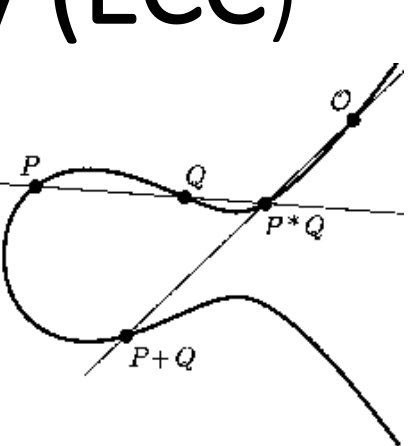
\includegraphics[width=45.15mm,height=122.66mm]{images/llm/page_001_img_01.png}%
\end{textblock*}

\newpage

% --- unit llm 2 ---
% === Halaman 2 (llm) ===

\textbf{Referensi:}

\begin{enumerate}
  \item Andreas Steffen, \textit{Elliptic Curve Cryptography}, Zürcher Hochschule Winterthur.
  \item Debdeep Mukhopadhyay, \textit{Elliptic Curve Cryptography}, Dept of Computer Sc and Engg IIT Madras.
  \item Anoop MS, \textit{Elliptic Curve Cryptography, an Implementation Guide}
\end{enumerate}

\newpage

% --- unit llm 3 ---
% === Halaman 3 (llm) ===

\section*{Teori Aljabar Abstrak}

\begin{itemize}
    \item Sebelum membahas ECC, perlu dipahami beberapa konsep aljabar abstrak yang mendasarinya.
\end{itemize}

\begin{itemize}
    \item Konsep aljabar abstrak:
    \begin{enumerate}
        \item Grup (\textit{group})
        \item Cincin (\textit{ring})
        \item Medan (\textit{field})
        \item Galois field
    \end{enumerate}
\end{itemize}

\newpage

% --- unit llm 4 ---
% === Halaman 4 (llm) ===

\section*{Grup}

\begin{itemize}
    \item Grup (\textit{group}) adalah sistem aljabar yang terdiri dari:
    \begin{itemize}
        \item sebuah himpunan $G$
        \item sebuah operasi biner $*$
    \end{itemize}
    sedemikian sehingga untuk semua elemen $a, b$, dan $c$ di dalam $G$ berlaku aksioma berikut:
    \begin{enumerate}
        \item \textit{Closure}: $a * b$ harus berada di dalam $G$
        \item Asosiatif: $a * (b * c) = (a * b) * c$
        \item Elemen netral: terdapat $e \in G$ sedemikian sehingga $a * e = e * a = a$
        \item Elemen invers: terdapat $a' \in G$ sedemikian sehingga $a * a' = a' * a = e$
    \end{enumerate}
    \item Notasi: $\langle G, *\rangle$
\end{itemize}

\newpage

% --- unit llm 5 ---
% === Halaman 5 (llm) ===

\begin{itemize}
  \item $\langle G, + \rangle$ menyatakan sebuah grup dengan operasi penjumlahan.
  \item $\langle G, \cdot \rangle$ menyatakan sebuah grup dengan operasi perkalian
\end{itemize}

Contoh-contoh grup:

\begin{enumerate}
  \item $\langle R, + \rangle$ : grup dengan himpunan bilangan riil dengan operasi $+$ \\
  $e = 0$ dan $a' = -a$
  
  \item $\langle R^*, \cdot \rangle$ : grup dengan himpunan bilangan riil tidak nol (yaitu, $R^* = R - \{ 0 \}$) dengan operasi kali $(\cdot)$ \\
  $e = 1$ dan $a' = 1/a = a^{-1}$
  
  \item $\langle Z, + \rangle$ dan $\langle Z, \cdot \rangle$ masing-masing adalah grup dengan himpunan bilangan bulat (integer) dengan operasi $+$ dan $\cdot$.
\end{enumerate}

\vfill
\begin{center}
  Rinaldi Munir/II4021 Kriptografi
\end{center}

\newpage

% --- unit llm 6 ---
% === Halaman 6 (llm) ===

4. $\langle Z_n, \oplus \rangle$ : grup dengan himpunan \textit{integer} modulo $n$, yaitu $Z_n = \{0, 1, 2, ..., n - 1\}$ dan $\oplus$ adalah operasi penjumlahan modulo $n$.

Contoh: $n = 5$, $Z_n = \{0, 1, 2, 3, 4\}$, $(3 \oplus 4) = (3 + 4) \pmod 5 = 2$

$\langle Z_p, \oplus \rangle$ : grup dengan himpunan \textit{integer} modulo $p$, $p$ adalah bilangan prima, yaitu $Z_p = \{0, 1, 2, ..., p - 1\}$ dan $\oplus$ adalah operasi penjumlahan modulo $p$.

$\langle Z_p^*, \otimes \rangle$ : dengan himpunan integer bukan nol, $p$ adalah bilangan prima, yaitu $Z_p^* = \{1, 2, ..., p - 1\}$ dan $\otimes$ adalah operasi perkalian modulo $p$.

\newpage

% --- unit llm 7 ---
% === Halaman 7 (llm) ===

\begin{itemize}
    \item Sebuah grup $\langle G, *\rangle$ dikatakan \textcolor{red}{grup komutatif} atau \textcolor{red}{grup abelian} (atau disingkat \textcolor{red}{abelian} saja) jika berlaku aksioma komutatif $a * b = b * a$ untuk semua $a, b \in G$.
    \item $\langle R, +\rangle$ dan $\langle R, \cdot\rangle$ adalah abelian
    \item $\langle Z, +\rangle$ dan $\langle Z, \cdot\rangle$ adalah abelian
    \item tetapi, $\langle M, \times\rangle$, dengan $M$ adalah himpunan matriks $2 \times 2$ dengan determinan $\neq 0$ bukan abelian (tanya kenapa?)
\end{itemize}

\vspace{10mm}

Ket: Abelian diambil dari kata ``abel'', untuk menghormati Niels Abel, seorang Matematikawan Norwegia (1802 -- 1829)

\newpage

% --- unit llm 8 ---
% === Halaman 8 (llm) ===

\textbf{Niels Henrik Abel} (5 August 1802 -- 6 April 1829) was a \href{https://en.wikipedia.org/wiki/Norwegian}{Norwegian} \href{https://en.wikipedia.org/wiki/Mathematician}{mathematician} who made pioneering contributions in a variety of fields. His most famous single result is the first complete proof demonstrating the impossibility of solving the \href{https://en.wikipedia.org/wiki/Quintic_equation}{general quintic equation} in radicals. This question was one of the outstanding open problems of his day, and had been unresolved for 250 years. He was also an innovator in the field of \href{https://en.wikipedia.org/wiki/Elliptic_function}{elliptic functions}, discoverer of \href{https://en.wikipedia.org/wiki/Abelian_function}{Abelian functions}. Despite his achievements, Abel was largely unrecognized during his lifetime; he made his discoveries while living in poverty and died at the age of 26.

Most of his work was done in six or seven years of his working life.\cite{1} Regarding Abel, the French mathematician \href{https://en.wikipedia.org/wiki/Charles_Hermite}{Charles Hermite} said: "Abel has left mathematicians enough to keep them busy for hundred years.\cite{1}\cite{2}"

\vspace{93.56mm}

Another French mathematician, \href{https://en.wikipedia.org/wiki/Adrien-Marie_Legendre}{Adrien-Marie Legendre}, said: "quelle t\^ete c\^elle du jeune Norv\^egien!" ("what a head the young Norwegian has!")\cite{3}

\vspace{10mm}

\begin{tabular}{ll}
Born & 5 August 1802 \\
& \href{https://en.wikipedia.org/wiki/Nedstrand}{Nedstrand}, \href{https://en.wikipedia.org/wiki/Norway}{Norway} \\
Died & 6 April 1829 (aged 26) \\
& \href{https://en.wikipedia.org/wiki/Froland}{Froland}, \href{https://en.wikipedia.org/wiki/Norway}{Norway} \\
Residence & Norway \\
Nationality & Norwegian \\
Fields & \href{https://en.wikipedia.org/wiki/Mathematics}{Mathematics} \\
Alma mater & \href{https://en.wikipedia.org/wiki/Royal_Frederick_University}{Royal Frederick University} \\
Known for & \begin{itemize}
\item Abel's binomial theorem
\item Abelian category
\item Abelian variety
\item Abelian variety of CM-type
\item Abel equation
\item Abel equation of the first kind
\item Abelian extension
\item Abel function
\item Abelian group
\item Abel's identity
\item Abel's inequality
\item Abel's irreducibility theorem
\item Abel--Jacobi map
\item Abel--Plana formula
\item Abel--Ruffini theorem
\item Abelian means
\item Abel's summation formula
\item Abel's theorem
\item Abel transform
\item Abel transformation
\item Abelian variety
\item Dual abelian variety
\end{itemize}
\end{tabular}

Sumber: Wikipedia

% deskripsi: Foto potret hitam putih Niels Henrik Abel
% bbox normalisasi: [0.4970, 0.3450, 0.6950, 0.6600]
\begin{textblock*}{41.58mm}(104.37mm,102.46mm)
\noindent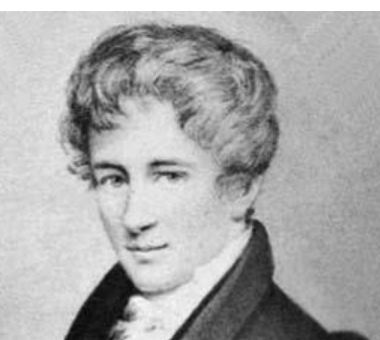
\includegraphics[width=41.58mm,height=93.56mm]{images/llm/page_008_img_01.png}%
\end{textblock*}

\newpage

% --- unit llm 9 ---
% === Halaman 9 (llm) ===

\section*{Medan (\textit{Field})}

\begin{itemize}
    \item Medan (\textit{field}) adalah system aljabar yang terdiri dari
    \begin{itemize}
        \item himpunan elemen (disimbolkan dengan F)
        \item operasi biner, yaitu penjumlahan (+) dan perkalian ($\cdot$).
    \end{itemize}

    \item Sebuah struktur aljabar $\langle F, +, \cdot \rangle$ disebut medan jika dan hanya jika:
    \begin{enumerate}
        \item $\langle F, + \rangle$ adalah grup abelian
        \item $\langle F - \{0\}, \cdot \rangle$ adalah grup abelian
        \item Operasi $\cdot$ menyebar terhadap operasi $+$ (sifat distributif)
    \end{enumerate}
    Distributif:
    \[
    \begin{aligned}
    x \cdot (y + z) &= (x \cdot y) + (x \cdot z) \\
    (x + y) \cdot z &= (x \cdot z) + (y \cdot z)
    \end{aligned}
    \]

    \item Jadi, sebuah medan memenuhi aksioma: \textit{closure}, komutatif, asosiatif, dan distributif
\end{itemize}

\newpage

% --- unit llm 10 ---
% === Halaman 10 (llm) ===

\begin{itemize}
    \item Contoh medan:
    \begin{itemize}
        \item medan bilangan bulat, $\langle\mathbb{Z}, +, .\rangle$
        \item medan bilangan riil, $\langle\mathbb{R}, +, .\rangle$
        \item medan bilangan rasional $(p/q)$, $\langle\mathbb{Q}, +, .\rangle$
    \end{itemize}

    \item Sebuah medan disebut berhingga (\textit{finite field}) jika himpunannya memiliki jumlah elemen yang berhingga.
    
    Jika jumlah elemen di dalam himpunan adalah $n$, maka notasinya $F_n$
    
    Contoh: $F_2$ adalah medan dengan elemen 0 dan 1

    \item Medan berhingga sering dinamakan juga \textcolor{red}{Galois Field}, untuk menghormati Evariste Galois, seorang matematikawan Perancis (1811 -- 1832)
\end{itemize}

\newpage

% --- unit llm 11 ---
% === Halaman 11 (llm) ===

\vspace{238.79mm}

\begin{center}\textcolor{red}{\textbf{Evariste Galois}}\end{center}

\vspace{60mm}

\begin{tabular}{ll}
Born & 25 October 1811 \\
& \textcolor{blue}{Bourgl-la-Reine}, \textcolor{blue}{French Empire} \\
\addlinespace[2mm]
Died & 31 May 1832 (aged 20) \\
& Paris, \textcolor{blue}{Kingdom of France} \\
\addlinespace[2mm]
Nationality & French \\
\addlinespace[2mm]
Fields & Mathematics \\
\addlinespace[2mm]
Known for & Work on the \textcolor{blue}{theory of equations} and \textcolor{blue}{Abelian integrals}
\end{tabular}

% deskripsi: Potret sketsa wajah Evariste Galois
% bbox normalisasi: [0.0600, 0.1080, 0.9400, 0.9120]
\begin{textblock*}{184.80mm}(12.60mm,32.08mm)
\noindent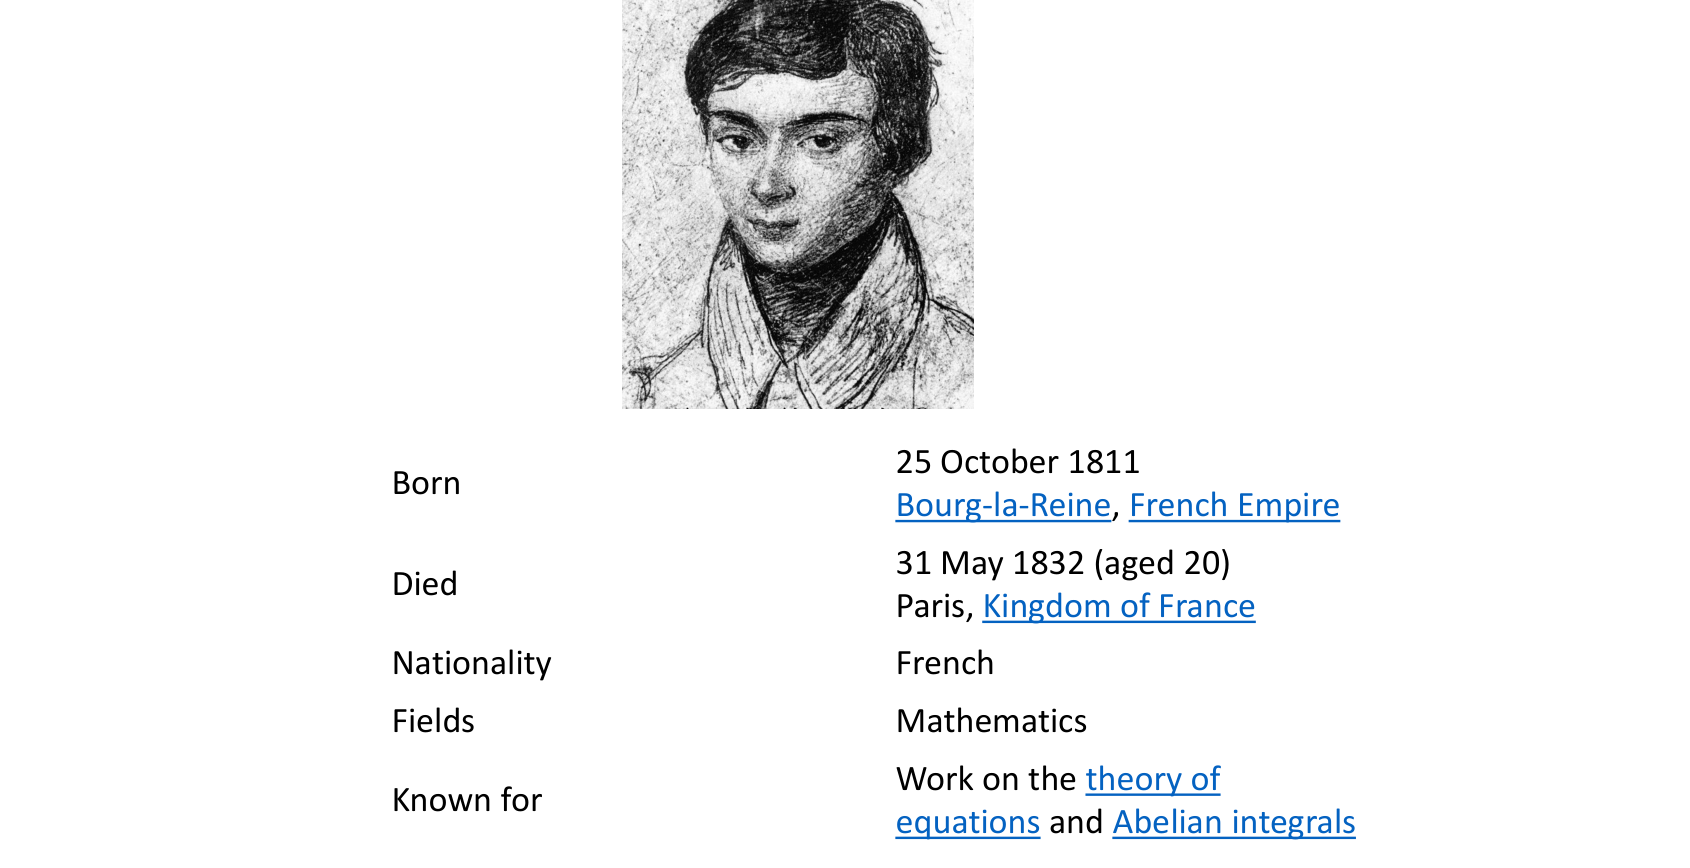
\includegraphics[width=184.80mm,height=238.79mm]{images/llm/page_011_img_01.png}%
\end{textblock*}

% bbox perkiraan otomatis: Potret sketsa wajah Evariste Galois

\newpage

% --- unit llm 12 ---
% === Halaman 12 (llm) ===

\section*{Medan Berhingga $F_p$}

\begin{itemize}
    \item Kelas medan berhingga yang penting adalah $F_p$, dengan $p$ adalah bilangan prima.
    \item $F_p$ adalah adalah medan berhingga dengan himpunan bilangan bulat $\{0, 1, 2, \dots, p-1\}$, $p$ bilangan prima, dan dua operasi yang didefinisikan sbb:
\end{itemize}

\begin{enumerate}
    \item \textbf{Penjumlahan}, dilakukan dalam modulus $p$
    \[
    \text{Jika } a, b \in F_p, \text{ maka } a + b = r, \text{ yang dalam hal ini}
    \]
    \[
    r = (a + b) \pmod p, \quad 0 \le r \le p - 1
    \]
    \item \textbf{Perkalian}, dilakukan dalam modulus $p$
    \[
    \text{Jika } a, b \in F_p, \text{ maka } a \cdot b = s, \text{ yang dalam hal ini}
    \]
    \[
    s = (a \cdot b) \pmod p, \quad 0 \le s \le p - 1
    \]
\end{enumerate}

\vfill
\begin{center}
    Rinaldi Munir/II4021 Kriptografi
\end{center}

\newpage

% --- unit llm 13 ---
% === Halaman 13 (llm) ===

\textbf{Contoh:} $\mathrm{F}_{23}$ mempunyai anggota $\{0, 1, 2, ..., 22\}$.
Contoh operasi aritmetika di dalam $\mathrm{F}_{23}$:
\[ 12 + 20 = 9 \quad (\text{karena } 12 + 20 = 32 \pmod{23} = 9) \]
\[ 8 \cdot 9 = 3 \quad (\text{karena } 8 \times 9 = 72 \pmod{23} = 3) \]

\newpage

% --- unit llm 14 ---
% === Halaman 14 (llm) ===

\section*{Medan Galois (Galois Field)}

\begin{itemize}
    \item Medan Galois adalah medan berhingga dengan $p^m$ elemen, $p$ adalah bilangan prima dan $m \ge 1$.
    \item Notasi: $GF(p^m)$
    \item Kasus paling sederhana: bila $m = 1 \rightarrow GF(p)$ atau $\text{F}_p$
    \item $GF(p)$ terdiri dari himpunan $\{0, 1, 2, ..., p-1\}$ dan operasi penjumlahan dan perkalian dilakukan di dalam modulus $p$.
\end{itemize}

\begin{enumerate}
    \item \textbf{Penjumlahan}, dilakukan dalam modulus $p$
    
    Jika $a, b \in GF(p)$, maka $a + b = r$, yang dalam hal ini $r = (a + b) \pmod p$, $0 \le r \le p - 1$
    
    \item \textbf{Perkalian}, dilakukan dalam modulus $p$
    
    Jika $a, b \in GF(p)$, maka $a \cdot b = s$, yang dalam hal ini $s = (a \cdot b) \pmod p$, $0 \le s \le p - 1$
\end{enumerate}

\vspace{10mm}

\centering Rinaldi Munir/II4021 Kriptografi

\newpage

% --- unit llm 15 ---
% === Halaman 15 (llm) ===

\vspace{47.52mm}

$p = 2 \rightarrow GF(2):$
\vspace{40mm}
$p = 3 \rightarrow GF(3):$

\vspace{65.34mm}

% deskripsi: Tabel penjumlahan dan perkalian untuk field Galois GF(2)
% bbox normalisasi: [0.2100, 0.2300, 0.6900, 0.3900]
\begin{textblock*}{100.80mm}(44.10mm,68.31mm)
\noindent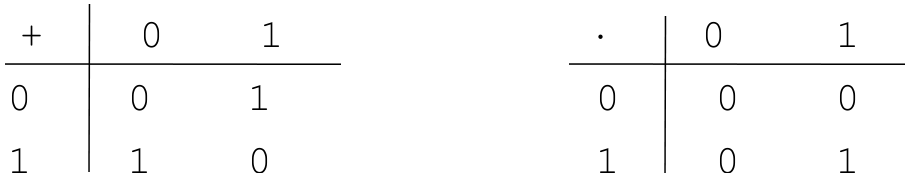
\includegraphics[width=100.80mm,height=47.52mm]{images/llm/page_015_img_01.png}%
\end{textblock*}

% deskripsi: Tabel penjumlahan dan perkalian untuk field Galois GF(3)
% bbox normalisasi: [0.2100, 0.5300, 0.7200, 0.7500]
\begin{textblock*}{107.10mm}(44.10mm,157.41mm)
\noindent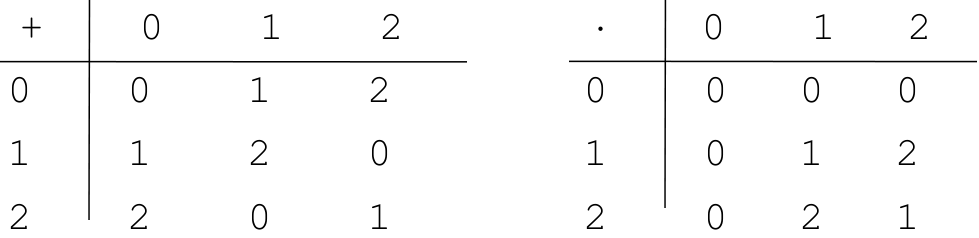
\includegraphics[width=107.10mm,height=65.34mm]{images/llm/page_015_img_02.png}%
\end{textblock*}

\newpage

% --- unit llm 16 ---
% === Halaman 16 (llm) ===

\begin{itemize}
    \item Contoh: Bentuklah tabel perkalian untuk GF(11), kemudian tentukan solusi untuk $x^2 \equiv 5 \pmod{11}$
\end{itemize}

\vspace{10mm}

\begin{align*}
    & x^2 \equiv 5 \pmod{11} \\
    & \text{Maka:} \\
    & x^2 = 16 \rightarrow x_1 = 4 \\
    & x^2 = 49 \rightarrow x_2 = 7
\end{align*}

\vspace{5mm}

Cara lain: cari elemen diagonal $= 5$, lalu ambil elemen mendatar atau elemen Vertikalnya (dilingkari).

\vspace{10mm}

\textcolor{red}{Sumber: Andreas Steffen, Elliptic Curve Cryptography} \\
\text{Rinaldi Munir/L4021 Kriptografi}

% deskripsi: Tabel perkalian Galois Field GF(11) dengan penandaan warna dan lingkaran untuk menunjukkan solusi x^2 = 5 mod 11.
% bbox normalisasi: [0.1800, 0.2300, 0.6100, 0.8800]
\begin{textblock*}{90.30mm}(37.80mm,68.31mm)
\noindent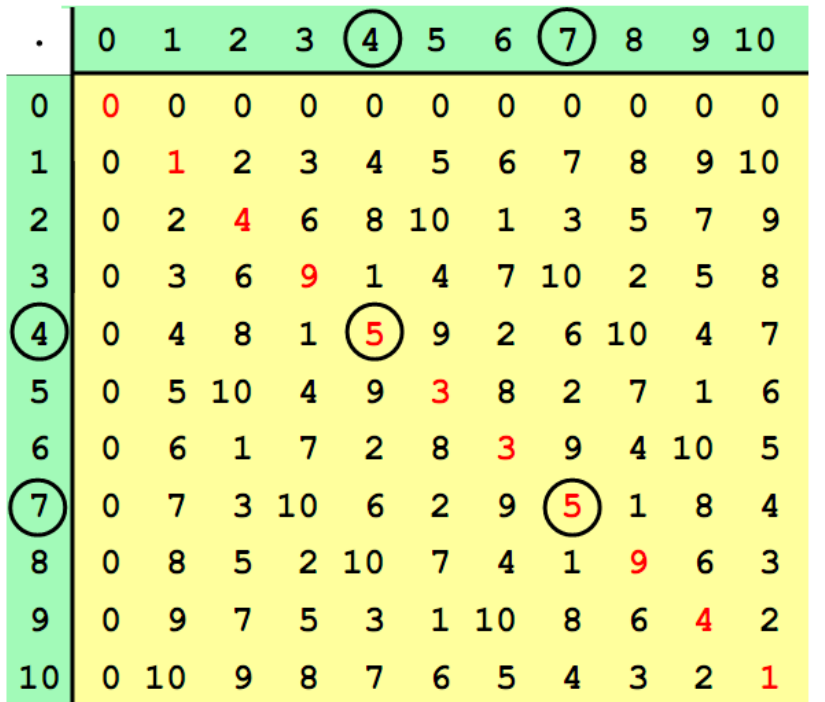
\includegraphics[width=90.30mm,height=193.05mm]{images/llm/page_016_img_01.png}%
\end{textblock*}

\newpage

% --- unit llm 17 ---
% === Halaman 17 (llm) ===

\section*{Galois Field GF($2^m$)}

\begin{itemize}
    \item Dari GF($p^m$), jika $p = 2$, maka GF($2^m$) disebut juga medan berhingga biner.
    \item GF($2^m$) atau $\text{F}_2^m$ adalah ruang vektor berdimensi $m$ pada GF(2). Setiap elemen di dalam GF($2^m$) adalah integer dalam representasi biner sepanjang maksimal $m$ bit.
    Contoh: GF($2^4$), GF($2^8$), dst
    \item String biner $b_{m-1}b_{m-2} \dots b_1b_0$, $b_i \in \{0,1\}$, dapat dinyatakan sebagai polinom
    \[ b_{m-1}x^{m-1} + b_{m-2}x^{m-2} + \dots + b_1x + b_0 \]
    \item Jadi, setiap $a \in \text{GF}(2^m)$ dapat dinyatakan sebagai
    \[ b_{m-1}x^{m-1} + b_{m-2}x^{m-2} + \dots + b_1x + b_0 \]
    \item Contoh: 1101 di dalam GF($2^4$) dapat dinyatakan sebagai polinom $x^3 + x^2 + 1$
    
    0101010111 di dalam GF($2^8$) dapat dinyatakan sebagai polinom $x^6 + x^4 + x^2 + x + 1$
\end{itemize}

\newpage

% --- unit llm 18 ---
% === Halaman 18 (llm) ===

\section*{Operasi aritmetika pada $\text{GF}(2^m)$}

Misalkan $a = (a_{m-1} \dots a_1 \ a_0)$ dan $b = (b_{m-1} \dots b_1 \ b_0) \in \text{GF}(2^m)$

\begin{itemize}
    \item \textbf{Penjumlahan:}
    \[ a + b = c = (c_{m-1} \dots c_1 \ c_0), \text{ yang dalam hal ini } c_i = (a_i + b_i) \pmod{2}, \ c \in \text{GF}(2^m) \]

    \item \textbf{Perkalian:}
    \[ a \cdot b = c = (c_{m-1} \dots c_1 \ c_0), \text{ yang dalam hal ini } c \text{ adalah sisa pembagian} \]
    polinom $a(x) \cdot b(x)$ dengan \textit{irreducible polynomial} derajat $m$, $c \in \text{GF}(2^m)$.
\end{itemize}

\textcolor{red}{\textbf{Note:} Sebuah polinom dikatakan tidak dapat direduksi (\textit{irreducible polynomial}) jika ia tidak dapat dinyatakan sebagai perkalian dari dua buah polinom lain (kecuali perkalian dengan 1 dan dirinya sendiri).

Polinom $x^2 + 1$ dan $x^4 + x + 1$ adalah \textit{irreducible} di dalam $\text{GF}(2^m)$, tetapi polinom $x^5 + x^2 + x + 1$ \textit{reducible} karena $x^5 + x^2 + x + 1 = (x^3 + x^2 + 1) \cdot (x^2 + 1)$}

\newpage

% --- unit llm 19 ---
% === Halaman 19 (llm) ===

\textbf{Contoh 1:} Misalkan $a = 00001101 = x^3 + x^2 + 1$ dan $b = 00000110 = x^2 + x$\
$a$ dan $b \in GF(2^8)$ \quad (dalam notasi Hex, $a = \text{'0D'}$ dan $b = \text{'06'}$)\

(i) $a + b = \text{'0D'} + \text{'06'} = (x^3 + x^2 + 1) + (x^2 + x) = x^3 + 2x^2 + x + 1 \pmod{2}$

\begin{align*}
\text{\color{red}Bagi tiap koefisien dengan 2, lalu ambil sisanya} \\
&= x^3 + 0x^2 + x + 1 \\
&= x^3 + x + 1 = 00001011 = \text{'0B'}
\end{align*}

Dalam representasi biner:

\begin{align*}
&00001101 \\
&00000110 + \\
&00001011 \rightarrow \text{sama dengan hasil operasi XOR}
\end{align*}

$\therefore a + b = 00001011 = a \text{ XOR } b$

\vspace{10mm}

\centering Rinaldi Munir/II4021 Kriptografi

\newpage

% --- unit llm 20 ---
% === Halaman 20 (llm) ===

\textbf{Contoh 2:} Misalkan $a = 01010111 = x^6 + x^4 + x^2 + x + 1$ dan $b = 10000011 = x^7 + x + 1$\
$a$ dan $b \in \text{GF}(2^8)$ (dalam notasi Hex, $a = \text{'57'}$ dan $b = \text{'83'}$)\
(i) $a + b = \text{'57'} + \text{'83'} = (x^6 + x^4 + x^2 + x + 1) + (x^7 + x + 1)$\
\begin{align*}$\\ = x^7 + x^6 + x^4 + x^2 + x + 2 \pmod{2} \quad \text{\color{red}Bagi tiap koefisien dengan 2,}\\ &\text{\color{red}lalu ambil sisanya}\\ = x^7 + x^6 + x^4 + x^2 + x + 0$\\ $= x^7 + x^6 + x^4 + x^2 + x = 11010100 = \text{'D4'}$\end{align*}\
Dalam representasi biner:
\begin{center}
\begin{tabular}{rl}
01010111 \\ $\underline{10000011} +$ \\ 11010100 $\rightarrow$ sama dengan hasil operasi XOR
\end{tabular}
\end{center}
$\therefore a + b = 11010100 = a \text{ XOR } b$

\vspace{10mm}
\begin{center}
\small Rinaldi Munir/II4021 Kriptografi
\end{center}

\newpage

% --- unit llm 21 ---
% === Halaman 21 (llm) ===

(ii) \begin{align* a \cdot b &= (x^6 + x^4 + x^2 + x + 1) \cdot (x^7 + x + 1) \\ &= x^{13} + x^7 + x^6 + x^{11} + x^5 + x^4 + x^9 + x^3 + x^2 + x^8 + x^2 + x + x^7 + x + 1 \pmod{2} \\ &= x^{13} + x^{11} + x^9 + x^8 + 2x^7 + x^6 + x^5 + x^4 + x^3 + 2x^2 + 2x + 1 \pmod{2} \\ &= x^{13} + x^{11} + x^9 + x^8 + 0x^7 + x^6 + x^5 + x^4 + x^3 + 0x^2 + 0x + 1 \\ &= x^{13} + x^{11} + x^9 + x^8 + x^6 + x^5 + x^4 + x^3 + 1 \end{align*}

Karena $m = 8$, maka hasil perkalian di atas direduksi menjadi derajat $< 8$ oleh \textit{irreducible polynomial}.

Contoh, algoritma Rijndael (AES) beroperasi dalam $\text{GF}(2^8)$ dan menggunakan \textit{irreducible polynomial} $f(x) = x^8 + x^4 + x^3 + x + 1$

\[ x^{13} + x^{11} + x^9 + x^8 + x^6 + x^5 + x^4 + x^3 + 1 \pmod{f(x)} = x^7 + x^6 + 1 = 11000001 \]

$\therefore a \cdot b = 11000001 = \text{'C1'}$

\newpage

% --- unit llm 22 ---
% === Halaman 22 (llm) ===

\vspace{50mm}

Jadi, $x^{13} + x^{11} + x^9 + x^8 + x^6 + x^5 + x^4 + x^3 + 1 \pmod{f(x)} = x^7 + x^6 + 1 = 11000001$

\vspace{10mm}

\centering Rinaldi Munir/II4021 Kriptografi

% deskripsi: Proses pembagian polinomial dalam aritmatika GF(2) yang menunjukkan langkah-langkah pembagian bersusun untuk mencari sisa pembagian.
% bbox normalisasi: [0.0600, 0.1080, 0.9400, 0.9120]
\begin{textblock*}{184.80mm}(12.60mm,32.08mm)
\noindent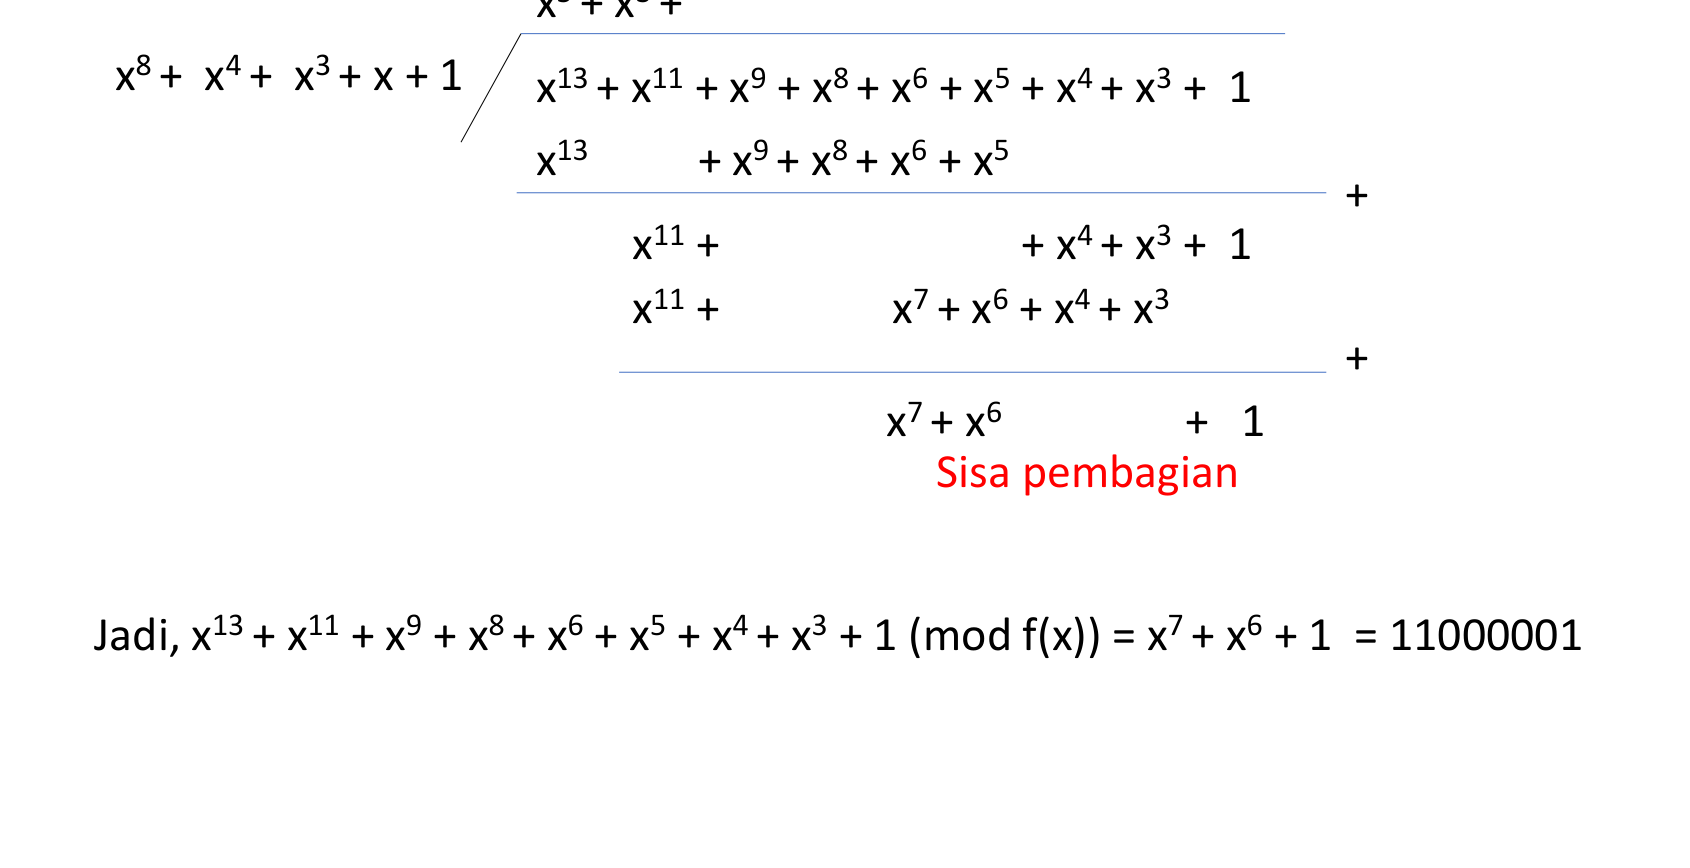
\includegraphics[width=184.80mm,height=238.79mm]{images/llm/page_022_img_01.png}%
\end{textblock*}

% bbox perkiraan otomatis: Proses pembagian polinomial dalam aritmatika GF(2) yang menunjukkan langkah-langkah pembagian bersusun untuk mencari sisa pembagian.

\newpage

% --- unit llm 23 ---
% === Halaman 23 (llm) ===

\vspace{135.73mm}

Contoh 3: \[ a \cdot b = (x^3 + x^2 + 1) \cdot (x^2 + x) = x^5 + 2x^4 + x^3 + x^2 + x \pmod 2) \\ = x^5 + x^3 + x^2 + x = 10110 \]

% deskripsi: Proses pembagian polinomial untuk mencari sisa pembagian (modulo) dari x^5 + x^3 + x^2 + x oleh x^4 + x + 1
% bbox normalisasi: [0.1800, 0.2400, 0.6070, 0.6970]
\begin{textblock*}{89.67mm}(37.80mm,71.28mm)
\noindent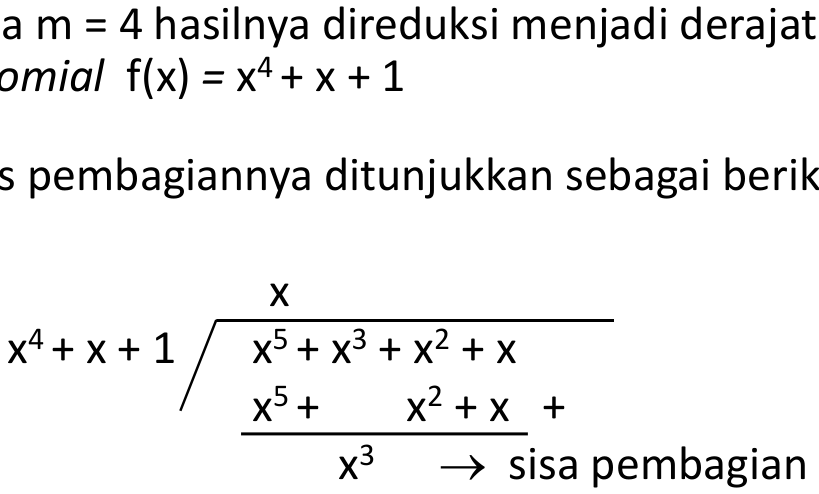
\includegraphics[width=89.67mm,height=135.73mm]{images/llm/page_023_img_01.png}%
\end{textblock*}

\newpage

% --- unit llm 24 ---
% === Halaman 24 (llm) ===

BERSAMBUNG

\vspace{50mm}

\begin{center}
// Rinaldi Munir/II4021 Kriptografi
\end{center}

\end{document}
